\scanpage{19}
\deleted{$\unsure{7|j|\mathbb Z}$} $b$\qquad $j$ et $j-1$ \unsure{unité|unités}

Cas $A$ local \uline{\unsure{normal ?}}
\[
\left\{\begin{aligned}
&j\text{ une unité, pas }j-1,\ (\text{pas idt nul})&
(1\unsure{-|+}j^{-1})^2\in A^6 A^{\unsure{*}}\\
&j-1\text{ une unité, } j\text{ pas (pas idt nul)}&
\left(\frac{\unsure{1|j}}{j-1}\right)^3\in A^6 A^*
\end{aligned}\right.
\]

% slanted
\margin{\uline{à vérifier} \uline{géométriquemt}}

\diagram{\begin{tikzcd}[ampersand replacement=\&,column sep=small]
{\text{Ext. Kummérienne du groupe }\mathbb Z/3}\arrow[r,leftrightarrow]\&j\equiv1\\
{\text{Ext. Kummérienne du groupe }\mathbb Z/2}\arrow[r,leftrightarrow]\&j\equiv0
\end{tikzcd}}

\[
\begin{aligned}
b^3=0,\ c\text{ inversible}\quad /\!/ &\ \text{si }\deleted{\unsure{a}} A\text{ sans élément nilpotents, alors l'invariant}\\
&\ \text{est }c\in A^*/A^{*(3)}\\
c^2=0,\ b\text{ inversible}\quad /\!/ &\ \text{si } A\ \text{ss élémt nilpotts,}\\
&\ \text{alors l'invariant est }b\in A^*/A^{*(2)}
\end{aligned}
\]

$1-$

\figure{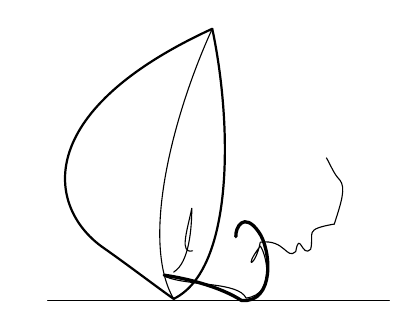
\begin{tikzpicture}[x=1cm,y=1cm,line cap=round,line join=round]
\draw[thin] (-.12,0)--(4.22,0);
\draw[thick] (1.97,3.45).. controls (-.36,2.38) and (-.12,1.15)..(.60,.66).. controls (.90,.45) and (1.28,.16)..(1.48,.02);
\draw (1.97,3.45).. controls (1.48,2.38) and (1.05,.76)..(1.48,.02);
\draw[thick] (1.97,3.45).. controls (2.22,2.28) and (2.26,.40)..(1.48,.02);
\draw[very thick] (1.36,.32).. controls (1.65,.28) and (2.08,.17)..(2.34,.00).. controls (2.77,-.04) and (2.72,.65)..(2.56,.87).. controls (2.37,1.14) and (2.26,.92)..(2.27,.81);
\draw (1.38,.30).. controls (1.68,.18) and (2.30,.24)..(2.40,.03).. controls (2.79,.08) and (2.65,.60)..(2.58,.69).. controls (2.35,.39) and (2.52,.42)..(2.58,.74).. controls (2.90,.78) and (2.91,.51)..(3.03,.62).. controls (3.08,.90) and (3.11,.53)..(3.22,.65).. controls (3.27,.86) and (3.12,.90)..(3.52,.97);
\draw (3.52,.97).. controls (3.61,1.25) and (3.67,1.43)..(3.59,1.53).. controls (3.51,1.61) and (3.47,1.73)..(3.42,1.81);
\draw (1.48,.36).. controls (1.68,.48) and (1.71,.93)..(1.71,1.17).. controls (1.65,.88) and (1.55,.59)..(1.72,.63);
\end{tikzpicture}}

\[
\begin{aligned}
\deleted{\unsure{j-1|j\equiv1}} \quad \left(\frac{t}{t-1}\right)^3 &\in O^6O^* &\quad&\text{\uline{marche pas}}\\
\left(\frac{t-1}{t}\right)^2 &\in O^6 O^{\unsure{*|\times}} &&\text{''}\qquad \sqrt[6]{\frac{t\deleted{\unsure{-1}}}{t-1}}
\end{aligned}
\]

\[
\sqrt[2]{\frac{t}{t-1}}\qquad \sqrt[3]{\frac{t-1}{t}}\qquad 1/2\qquad 1/3
\]

\figure{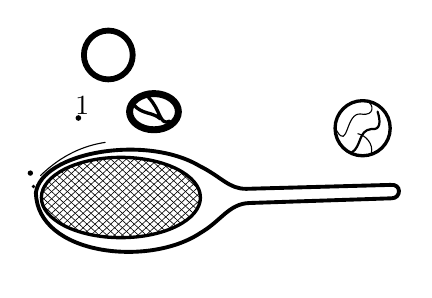
\begin{tikzpicture}[x=1cm,y=1cm,line cap=round,line join=round]
% crop-candidate: scan 19
\draw[line width=2.1pt] (1.02,2.66) circle (.31);
\draw[line width=2.5pt] (1.60,1.94) ellipse (.31 and .23);
\draw[very thick] (1.34,2.03).. controls (1.45,1.90) and (1.58,1.94)..(1.68,1.85) (1.53,2.12).. controls (1.68,1.98) and (1.67,1.75)..(1.80,1.82);
\draw[line width=1.2pt] (4.25,1.73) circle (.35);
\draw (3.92,1.70).. controls (4.07,1.44) and (4.03,1.94)..(4.23,1.91).. controls (4.41,1.88) and (4.39,2.04)..(4.31,2.07);
\draw[thick] (4.11,1.42).. controls (4.24,1.50) and (4.19,1.70)..(4.36,1.72).. controls (4.48,1.70) and (4.48,1.82)..(4.44,1.94);
\draw (4.19,1.66).. controls (4.29,1.64) and (4.39,1.53)..(4.36,1.41);
\draw[line width=1.4pt] (.10,.91).. controls (.17,1.42) and (1.49,1.66)..(2.18,1.25).. controls (2.46,1.11) and (2.55,.96)..(2.77,.96)--(4.60,1.01).. controls (4.75,1.03) and (4.74,.84)..(4.62,.84)--(2.81,.78).. controls (2.55,.77) and (2.45,.55)..(2.19,.40).. controls (1.53,-.04) and (.12,.12)..(.10,.91);
\draw[very thick] (1.18,.85) ellipse (1.01 and .51);
\begin{scope}
\clip (1.18,.85) ellipse (1.01 and .51);
\foreach \x in {-1,-.90,...,3.4}{\draw[line width=.22pt] (\x,.19)--++(1.36,1.25);\draw[line width=.22pt] (\x,.19)--++(-1.36,1.25);}
\end{scope}
\draw (.16,1.13).. controls (.44,1.40) and (.72,1.51)..(.98,1.55);
\fill (.03,1.16) circle (.034) (.07,.99) circle (.024) (.64,1.86) circle (.036);
\node at (.69,2.02) {$1$};
\end{tikzpicture}}

\[
\lambda^{3/6}\cdot\lambda^{\unsure{-2/6|-1/6}}=\lambda^{1/6}
\qquad \frac{-27c^{\unsure{2}}}{b^3-27c^2}=j
\]
\[
\deleted{\unsure{\sqrt[6]{t}}}\qquad s^6=\frac{t}{t-1}\qquad \frac{b^3}{c^2}=j\qquad 27c^2(j-1)=b^3j
\]

\[
\begin{array}{ccc}L&L^2&L^3\\&b&c\end{array}
\qquad
\begin{aligned} b^{\deleted{\unsure{3}}}&=27\frac{j-1}{j}\\ c&=27\frac{j-1}{j}\end{aligned}
\qquad \boxed{\frac{b^3}{c^2}=27\frac{j-1}{j}}
\]

% slanted
\margin{\unsure{$L_m-L-$}}

\figure{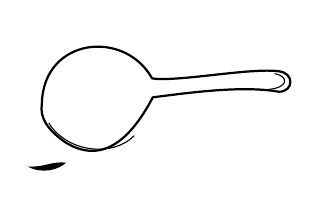
\begin{tikzpicture}[x=1cm,y=1cm,line cap=round,line join=round]
\draw[thick] (.00,.67).. controls (.02,1.51) and (1.05,1.62)..(1.40,.99).. controls (1.71,.94) and (2.66,1.13)..(3.01,1.08).. controls (3.21,1.06) and (3.20,.82)..(3.01,.82).. controls (2.52,.91) and (1.75,.79)..(1.41,.75).. controls (1.11,.18) and (.74,-.11)..(.28,.19).. controls (.08,.34) and (-.03,.48)..(.00,.67);
\draw (.09,.42).. controls (.34,.03) and (.92,.00)..(1.17,.26) (2.88,.85).. controls (3.12,.87) and (3.15,1.01)..(2.96,1.05);
\fill (-.18,-.13).. controls (.04,-.14) and (.12,-.06)..(.31,-.08).. controls (.21,-.17) and (.01,-.23)..(-.18,-.13);
\end{tikzpicture}}

\[
\boxed{x^3+27\frac{\unsure{j|t}-1}{j}(x+1)=0}
\]

\deleted{$\unsure{\mathrm{Hom}(E,}$}\quad $f_*(\check E)$

\diagram{\begin{tikzcd}[ampersand replacement=\&]
\underline{\mathrm{Hom}}_O(E,\underline O)\\
\mathrm{Hom}_{\underline A}(E,\underline A)\times\mathrm{Hom}_{\underline O}(\underline A,\underline O)\arrow[u]
\end{tikzcd}}
% archive sheet number: 18
